\documentclass[a4paper]{article}
\usepackage[utf8]{inputenc}
\usepackage[spanish]{babel} 
\renewcommand{\spanishtablename}{Tabla} 
\spanishdecimal{.}
\usepackage{verbatim}
\usepackage{amssymb}
\usepackage{subcaption}
\usepackage{wrapfig}
\usepackage{graphicx}
\usepackage{hyperref}
\usepackage{mathtools}
\usepackage{float}
\setlength{\parskip}{\baselineskip} 
\usepackage{pdfpages}

\begin{document}

\begin{titlepage}
\paragraph{}

\begin{center}
\vspace*{0.10in}
\begin{figure}
\raggedleft

\includegraphics[scale=0.12]{unam.png}
\hspace{7.2cm}
\raggedright
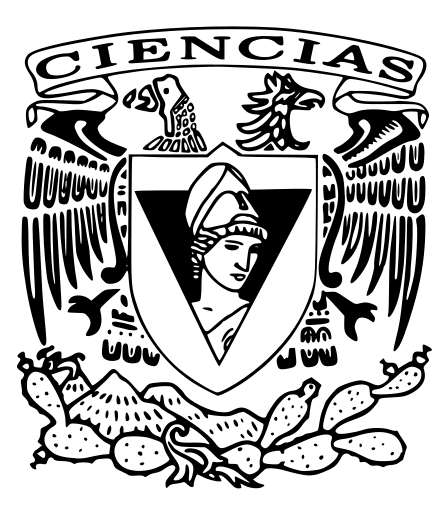
\includegraphics[scale=0.15]{fac.png}    
\end{figure}
\vspace*{0.5in}
UNIVERSIDAD NACIONAL AUTÓNOMA DE MÉXICO\\
\vspace*{0.2in}
FACULTAD DE CIENCIAS \\
\vspace*{0.5in}
\begin{large}
Laboratorio de Calor, Ondas y Fluidos\\
\end{large}
\vspace*{0.2in}
\begin{Large}
\textbf{Práctica 7} \\
\textbf{Principio de Arquímides.} \\
\end{Large}
\vspace*{0.3in}
\vspace*{0.3in}
\rule{80mm}{0.1mm}\\
\vspace*{0.1in}
\begin{large}
Profesor:  Quintanar Robles, Luis  \\
Ayudante: Quintanar Cortés, Luis Enrique \\
Mesa 1\\
Fecha de la práctica: 1 de octubre de 2019.\\
Alumnos: León Arenal Sebastian.\\
Robledo Ibarra Emiliano. \\
Toledo Castañeda, Akim Tarik.\\

\end{large}
\end{center}
\end{titlepage}



\section*{Resumen.}

El objetivo de las práctica fue verificar la veracidad y consecuencias del principio de Arquímedes para dos medios distintos. En ambos se buscó una relación entre el cambio en la masa y el producto de la densidad del fluido y el volumen desplazado de un líquido. El primero consistió en un sistema de volumen variable. Se encontró que, bajo el postulado del principio de Arquímedes, una equivalencia entre la fuerza de empuje producida por el cambio de volumen con respecto al cambio en el peso medido por una balanza. Se encontró una diferencia promedio entre $\Delta W$ y $F_{E}$ de $0.44\pm0.2N$ con lo cual se consideró una separación razonable que, aunque mejorable, habla de que están relacionadas estas dos fuerzas y el principio de Arquímedes lo modela adecuadamente. En el segundo se midieron cambios producidos por objetos regulares que eran sumergidos en líquidos, para este segundo se observó que en efecto son muy similares, sin embargo ocurrió que las incertidumbres al ser tan grandes opacan el resultado, es por ello por lo que se propuso una medición de volúmenes ya sea aprovechando las medidas de los objetos o con probetas mas sensibles.


\section*{Introducción.}
Arquímedes propuso un principio universal para los fluidos y como estos actúan sobre un cuerpo dentro del mismo: \textit{Todo cuerpo total o parcialmente sumergido en un fluido sufre un empuje de abajo arriba por una fuerza de magnitud igual al del peso del fluido que desaloja.} [1] Que matemáticamente se expresa como:

\begin{equation}
    F_E = \rho g V
\end{equation}

De esta forma, con este principio es posible explicar teóricamente por qué un barco flota o una piedra se hunde. Pero ¿por qué un cuerpo aparenta tener menos peso al medirlo dentro de un fluido como el agua? Dentro del fluido el cuerpo experimenta una fuerza atractiva hacia el centro del planeta, su  peso, además según Arquímedes al permanecer dentro del fluido, el cuerpo experimenta una fuerza que va en sentido opuesto al peso [debida al fluido que rodea al cuerpo, de tal forma que el peso del objeto en un fluido se ve afectado por las fuerzas que su exterior imprime sobre el mismo].

En esta práctica se busca verificar la relación entre el cambio del peso $W$ con la fuerza de empuje $F_{E}$ para el primer experimento y en el segundo, la relación entre el cambio de la masa $\delta m$ con el volumen desplazado $V$ además de comprobar que tan acertadas son estas relaciones para cada uno de los experimentos el fluido de la atmósfera (aire) y para tres líquidos distintos; para poder hacerlo se observó la diferencia entre las fuerzas que forman parte del sistema a analizar, es decir se obtendrá el cambio en el peso de un objeto antes y después de estar sometido a los efectos inherentes del fluido y posteriormente se calculó la fuerza propuesta por Arquímedes del sistema sobre el que actúa el aire y los fluidos. Para eficientar y simplificar las mediciones se supuso que el contenedor de aire (botella con válvula) tiene una fuerza de empuje despreciable por lo cual el globo es quien la expresa directamente, también se utilizó la hipótesis sobre un sistema hermético donde no hubo pérdida de masa con el exterior; usando estas hipótesis sólo se restringe el fluido a medir y se acota la fuerza que se quiere medir, de este modo la práctica se restringe a un lugar tan alto sobre el nivel del mar como la CDMX y al aire de la misma, además para el segundo experimento se utilizó la hipótesis adicional de que el hilo amarrado a los objetos,no tiene volumen.

\section*{Procedimiento.}
\subsection*{Procedimiento experimental 1}
Para el apartado de construcción del dispositivo se dividió en dos partes; en cuento al primero, se construyó un sistema de volumen variable con una botella de plástico de forma que se pudiese contener un volumen fijo, un globo receptor y una llave de tres vías. Para poder contener aire dentro de la botella se utilizó un compresor de aire. La segunda parte mediría el volumen suministrado a la botella y, en consecuencia, al globo. Para ello se construyó una cuba hidro-neumática con un contenedor de agua, una probeta con capacidad para un litro, una probeta de vidrio, una manguera, una jeringa y una llave de tres vías como se muestra en la Figura 1. 

\begin{figure}[H]
    \centering
    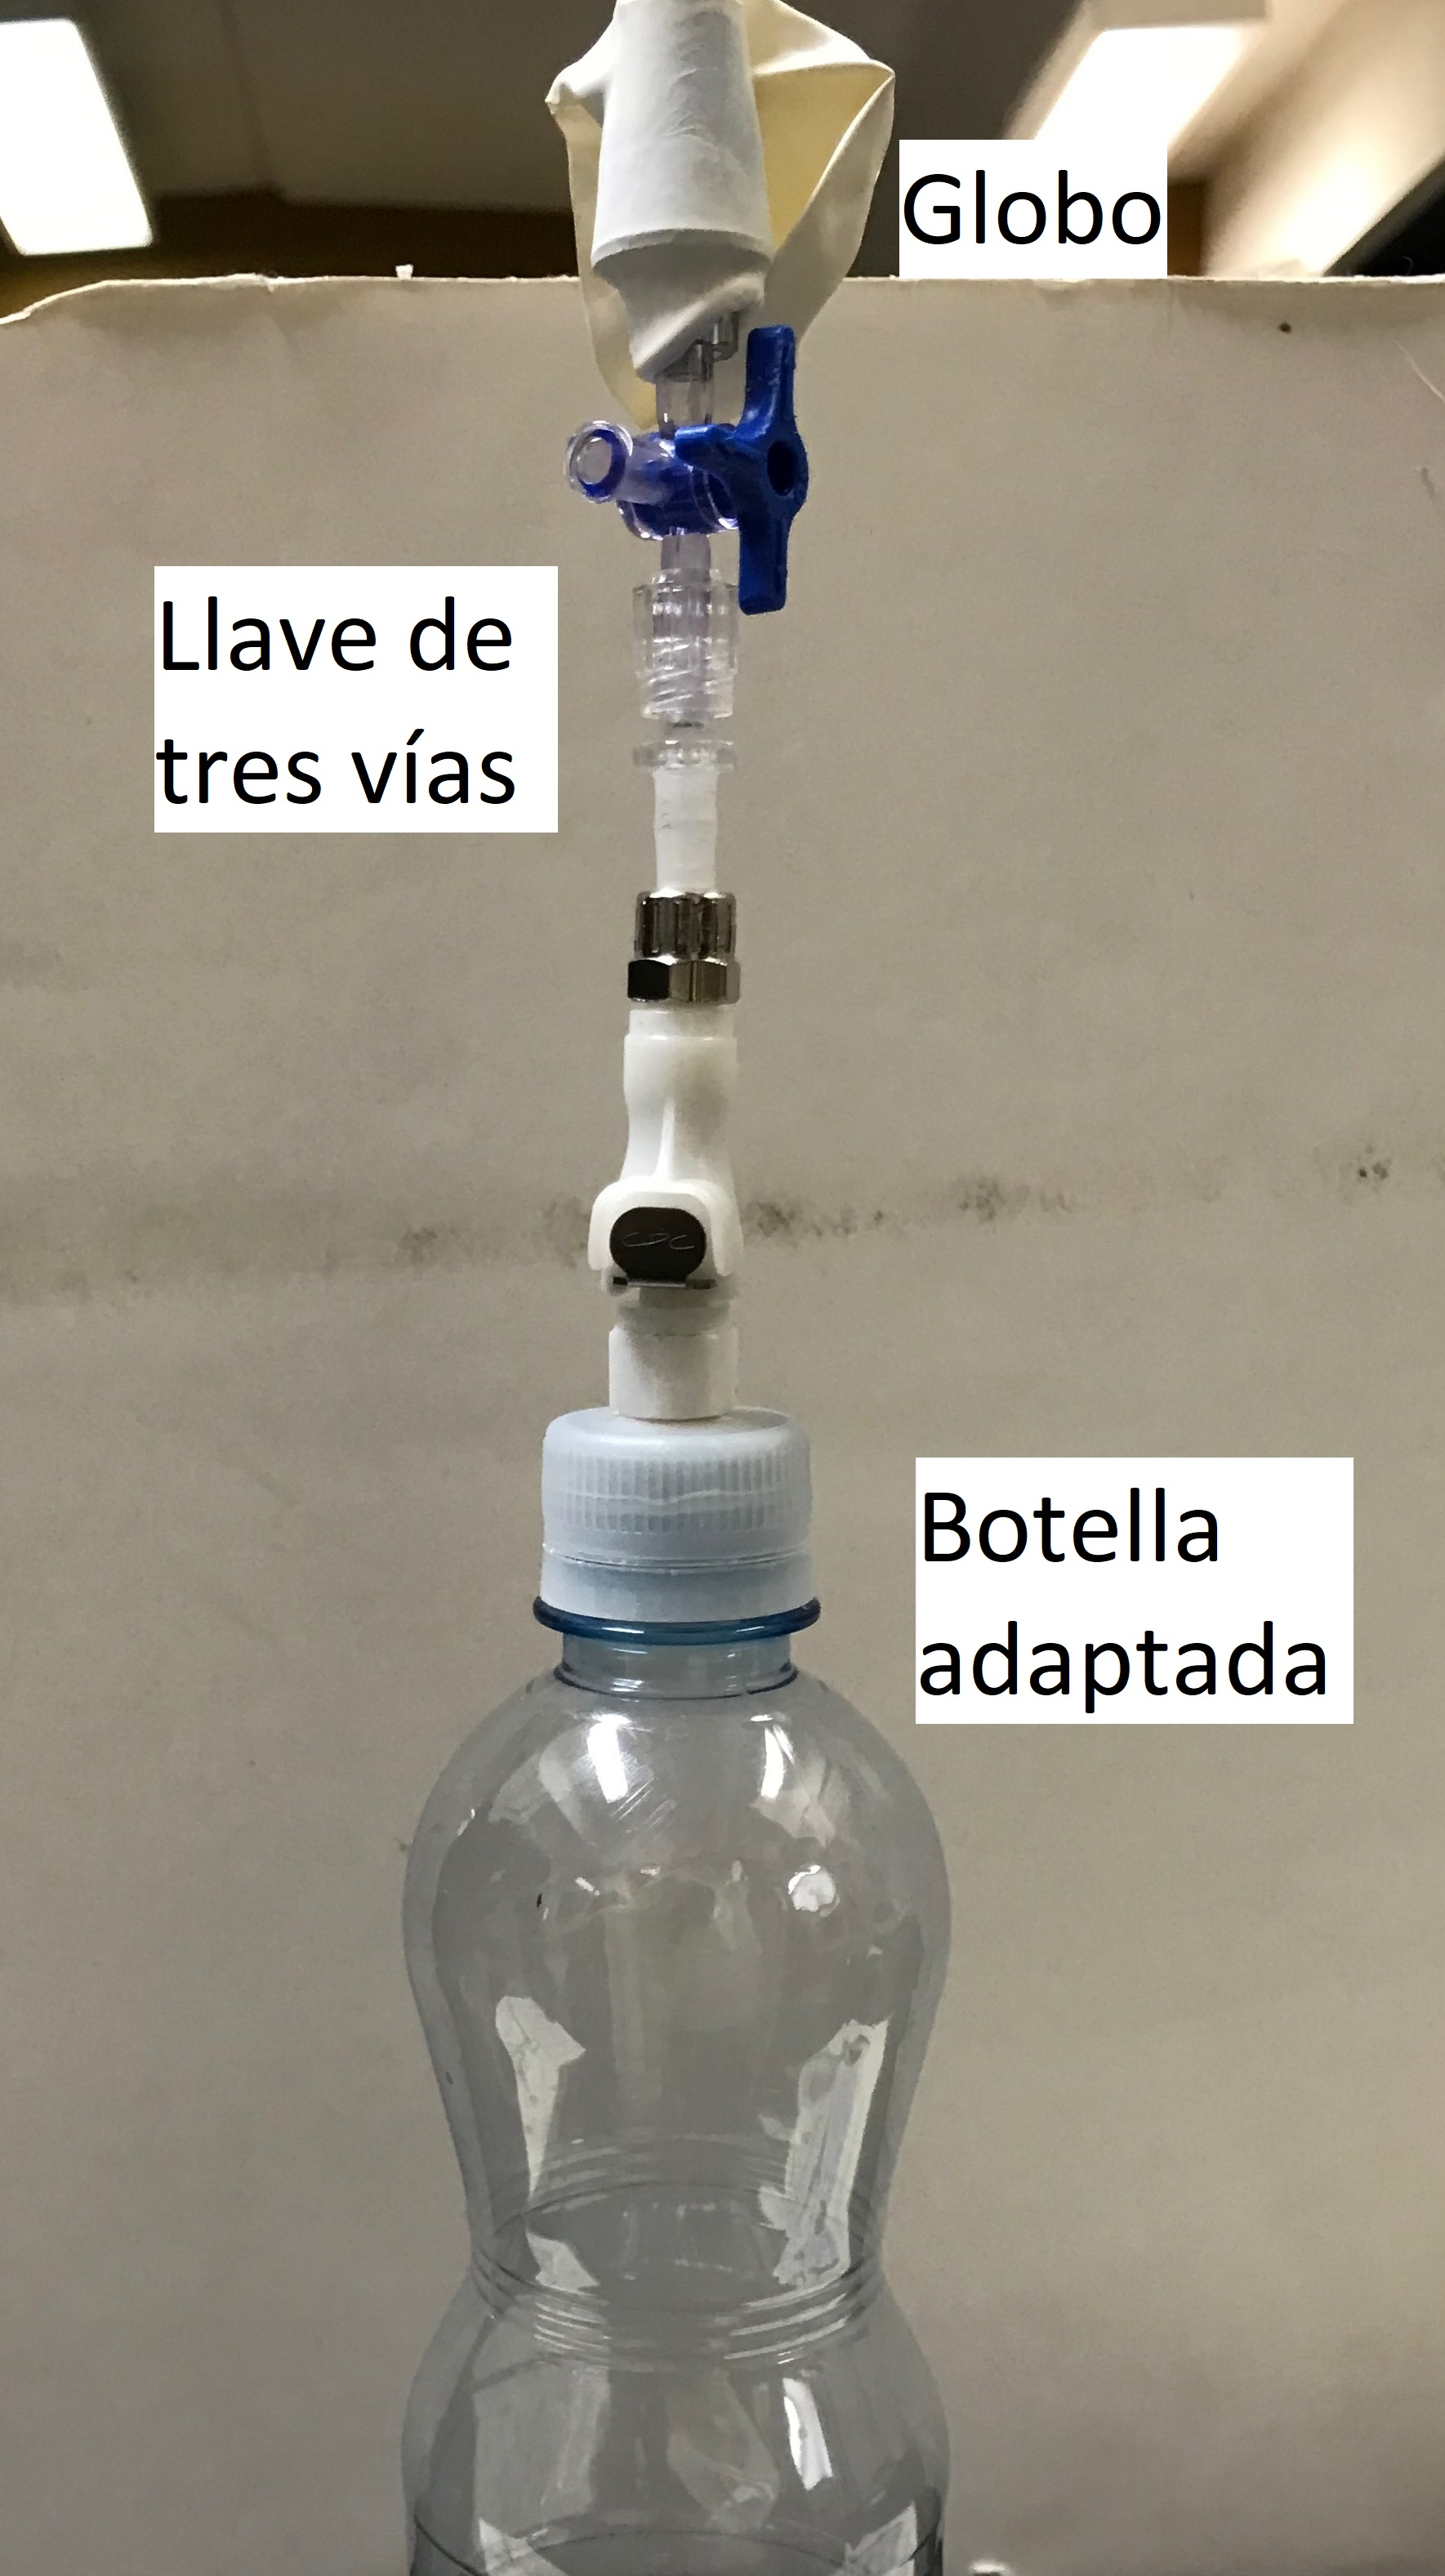
\includegraphics[width=5 cm]{Botella-Globo.JPG}
    \caption{Sistema de volumen variable}
\end{figure}

Para la medición se llenó el primer sistema con aire del compresor y se selló de modo que la llave de tres vías no permitiera el flujo de aire hacia el globo. Con ayuda de una balanza, se obtuvo la masa inicial del sistema con el globo sin aire ($m_{i}$). Luego, con ayuda de la llave de tres vías, se modificó el flujo de aire para permitir que el aire pasara libremente de la botella al globo (como consecuencia este se infló). Nuevamente se colocó el sistema, esta vez con el globo inflado, sobre la balanza para obtener su masa final ($m_{f}$).

La mínima resolución de la balanza utilizada es de $0.01 g$ por lo que se le asoció a todos los datos de masa una incertidumbre de $s_{W} = \pm 0.005 g$

Para calcular el incremento volumétrico del globo se utilizó una cuba hidro-neumática. Se separó el globo (unido con su llave de tres vías) del sistema para suministrar volumen, posteriormente se conectó la llave de tres vías con el globo a la cuba hidro-neumática y se orientaron las llaves de tres vías para que el aire saliera del globo y entrara a la probeta; de este modo, el volumen de agua dentro de la probeta se vio desplazado por el volumen de aire dentro del globo. Se registró esta diferencia de volumen como $V_{a}$.

La mínima resolución de la probeta utilizada es de 10 ml, a los datos volumétricos se les asignó una incertidumbre de $s_{V} = \pm 5ml$; en algunos casos fue necesario detener el flujo de aire del globo a la probeta, utilizar una bomba de vacío para elevar la columna de agua dentro de la probeta y volver a permitir el flujo del aire. Es decir, algunas mediciones requirieron de una doble medida y, por lo tanto, fueron sujetas al doble de incertidumbre $s_{V} = \pm 10ml$.

\begin{figure}[H]
    \centering
    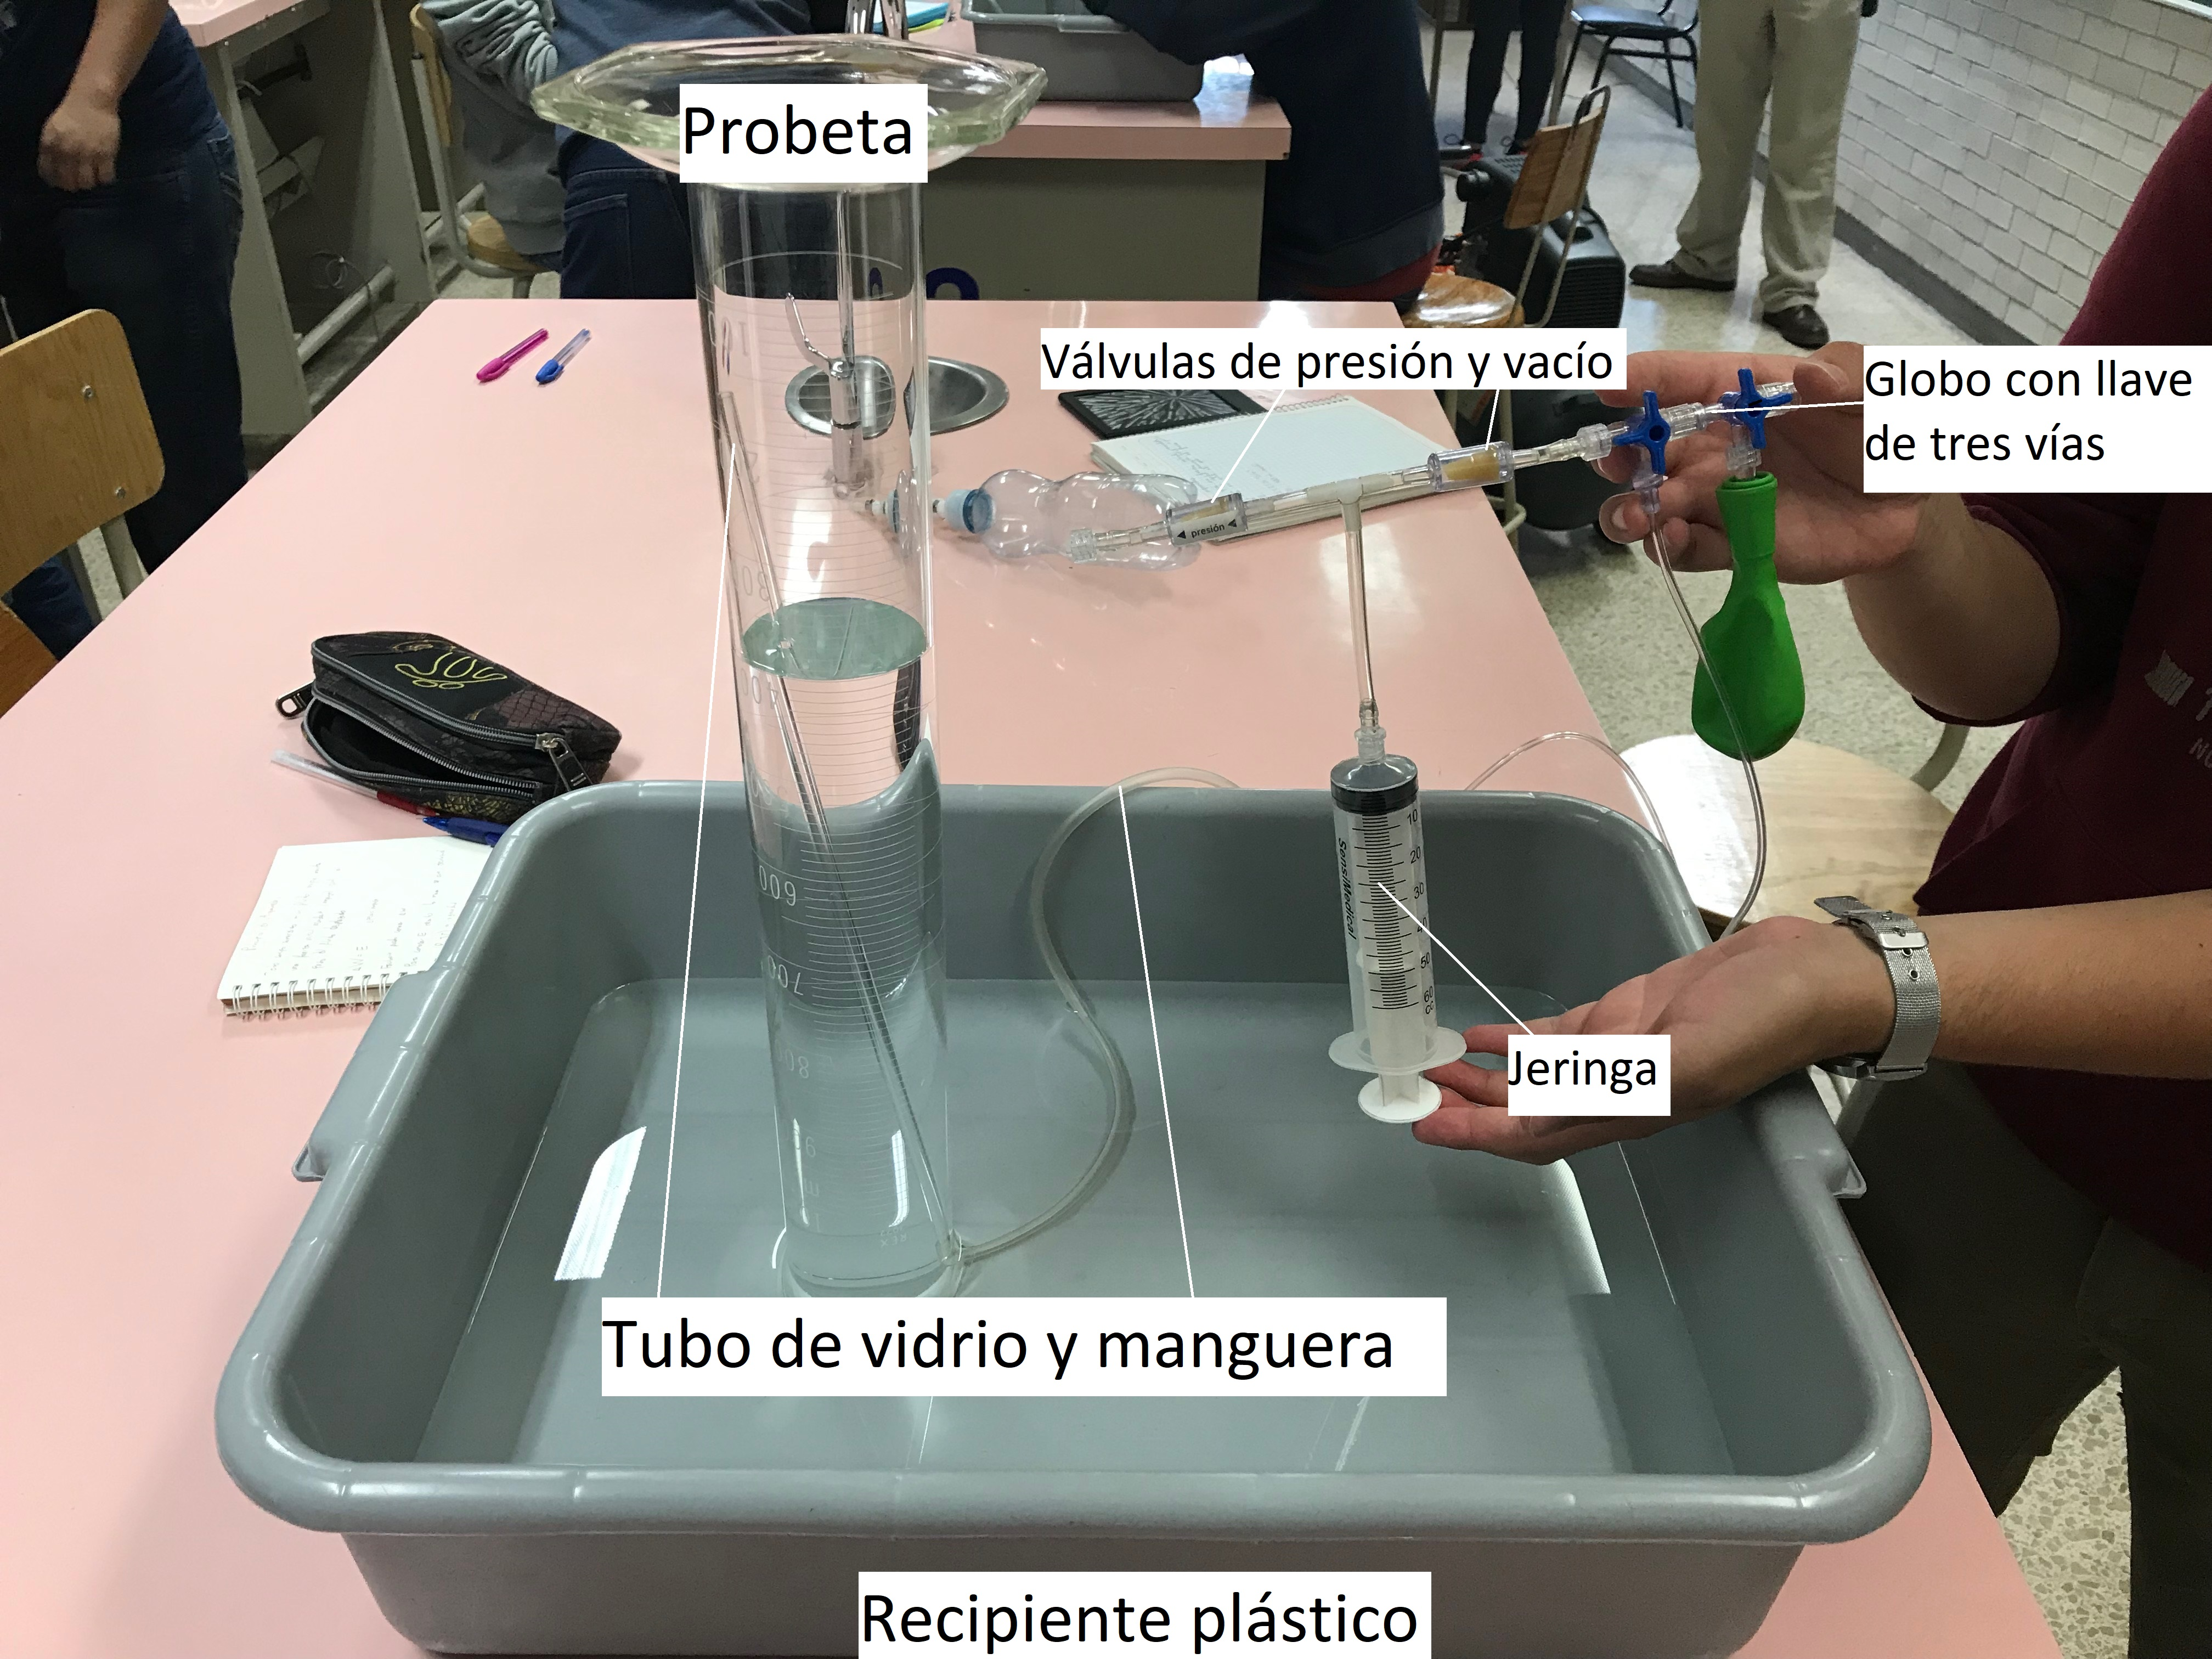
\includegraphics[width=9cm]{Sistema.JPG}
    \caption{Cuba hidro-neumática}
\end{figure}

Para el tratamiento de datos, se aclara que después de obtener las masas, estas se restaron obteniendo el valor $\Delta m$ que es el resultado de medir antes y después de soltar el aire al globo que estaba contenido en la botella; con el dato de la diferencia se calculó el peso de diferencia (definido como $\Delta m * g_{F.C.}$) denotado con $\Delta W$. Por otra parte la fuerza de empuje $F_{E}$ definida como el peso del volumen desplazado se calculó gracias al dato proporcionado por la probeta (volumen contenido en el globo), la gravedad (constante) y la densidad del aire.

Posteriormente, se compararon la diferencia de pesos y la fuerza de empuje para corroborar la relación $\Delta W = F_{E}$.

\subsection*{Procedimiento experimental 2}
En este segundo experimento se llenaron, parcialmente, tres probetas de medio litro con shampoo, glicerina y aceite (un líquido por probeta). Se colocó cada probeta en una balanza para obtener la masa de la probeta con su líquido. Con un soporte universal, una pinza de tres dedos y una nuez, se construyó una grúa primitiva para colgar objetos. Utilizando hilo se amarró un objeto a la pinza de tres dedos para quedar colgando. Se colocó la balanza a un lado del soporte; se colocó una probeta sobre la balanza y, finalmente, se alinearon la boca de la probeta y el objeto colgado de la pinza.

\begin{figure}[H]
    \centering
    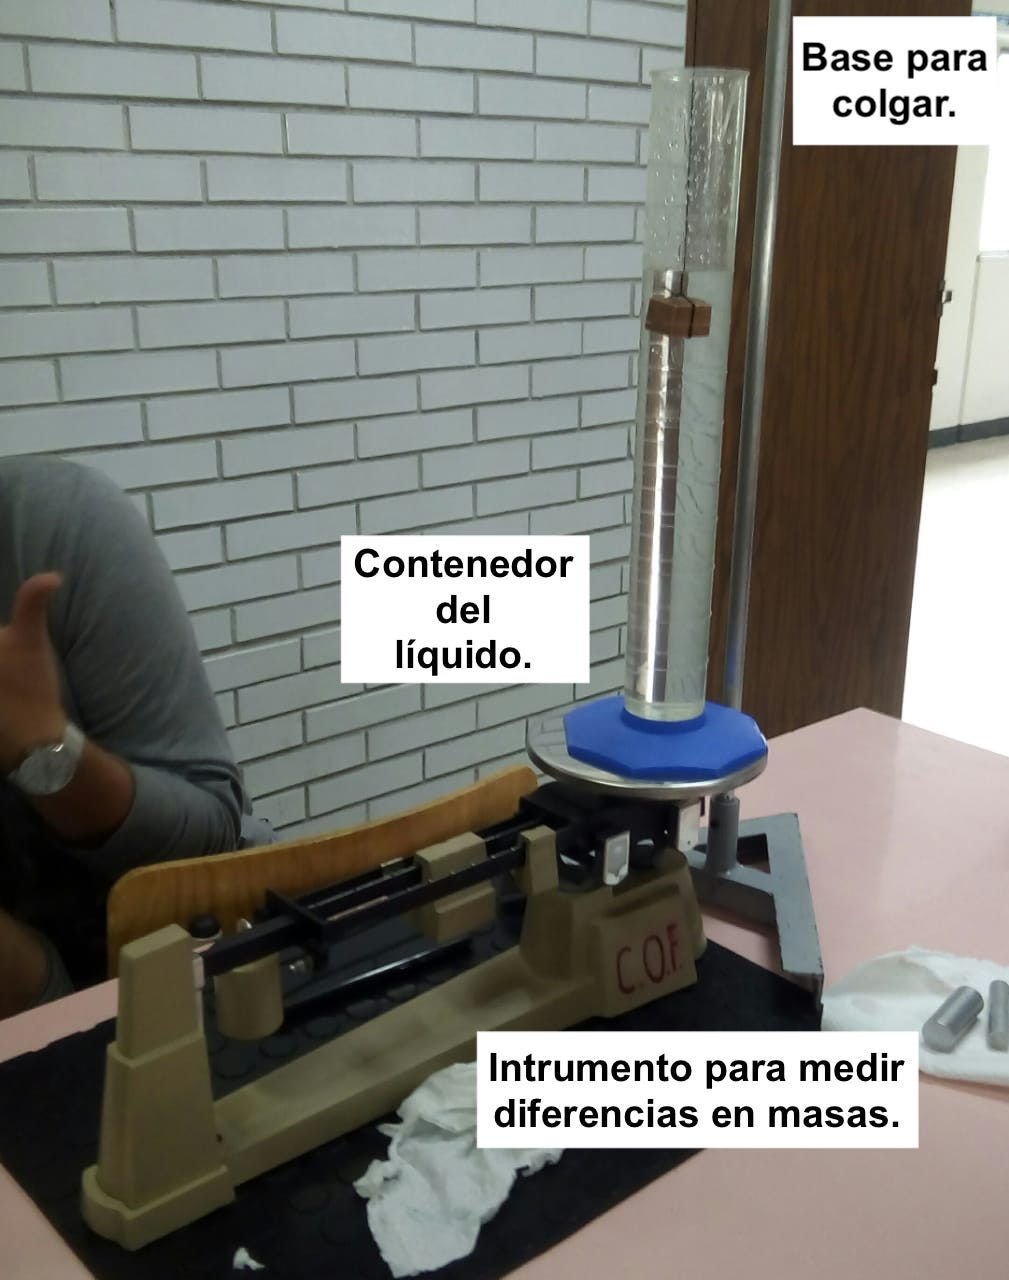
\includegraphics[width=7cm]{sis2.jpeg}
    \caption{Partes principales del sistema para la medición del segundo experimento.}
\end{figure}

Para cada medición y  por cada objeto primero se midió el volumen inicial de la probeta $V_i$ y el peso de la probeta con líquido dentro $m_i$. Se sumergió el objeto y se midieron las mismas variables de forma que se obtuvo un volumen final $V_f$ y una masa final $m_f$.
Se procuró que cada objeto colgado contara con el menor tramo de hilo, que quedase inmóvil dentro del líquido y que dentro no entrase en contacto con las paredes del contenedor. Se contó con una balanza que se calibró por medición de ser necesario y se procuró no intervenir con el objeto sumergido para la medición de su masa final.

El experimentó contó con una medida de reproducibilidad, se compararon los valores con un dinamómetro que sostuvo al objeto. Se observó que cada fuerza predicha por la fuerza de empuje y el cambio en el dinamómetro coincidían; una vez realizadas las pruebas y comprobada la reproducibilidad, se retiró el dinamómetro y se continuó el experimento sin él.

Referente a la incertidumbre, se catalogaron en dos tipos: directas e indirectas. En el caso de las directas se obtuvieron de la medición de masa inicial y final ($m_i$ y $m_f$) con una incertidumbre de $0.05 g$, los volúmenes inicial y final ($V_i$ y $V_f$) con incertidumbre de $2 mL$; para las medidas indirectas, como el cambio de volumen $\Delta V$, se utilizó la incertidumbre $4 mL$ ya que proviene de la resta de dos datos con la misma incertidumbre y a la diferencia de masas $\Delta m$ se le asignó $0.1 g$.

Una vez obtenidos los datos y asociadas las incertidumbres, se calculó la densidad de cada fluido utilizando $\Delta W=F_{E}=\rho_{l}\Delta V g$. La incertidumbre asociada a las densidades obtenidas se obtuvo con: $$\delta \rho = \frac{(\delta \Delta W *\Delta V)+(\delta \Delta V *\Delta W)}{(\delta \Delta V)^{2}}$$

%%%%%%%%%%%%%%%%%%%%%%%%%%%%%%%%%%%%%%%%%%%%%%%%%%%%%%%%%%%%%%%%%%%%%%%%
\section*{Resultados.}
\subsection*{Resultados del experimento 1}
A continuación se muestran los datos medidos del sistema globo-botella, se denota como la masa inicial $m_i$ a aquella sin haber liberado el aire al globo (es decir, con el globo desinflado), la masa final como $m_f$ a la masa registrada después de liberar el aire (con el globo inflado) y el volumen de aire $V_a$ al volumen medido en mL con la probeta en la cuba hidro-neumática.

\begin{table}[H]
  \centering
    \begin{tabular}{|c|c|c|c|} \hline
     & Masa i. ($m_i$) [gr] & Masa f. ($m_f$) [gr] & Vol. ($V_a$) [mL] \\ \hline
    1     & 53.750$\pm0.005$ & 53.650$\pm0.005$ & 110.$\pm5$ \\ \hline
    2     & 54.400$\pm0.005$ & 53.680$\pm0.005$ & 920$\pm10$ \\ \hline
    3     & 54.490$\pm0.005$ & 53.670$\pm0.005$ & 960$\pm10$ \\ \hline
    4     & 54.780$\pm0.005$ & 53.680$\pm0.005$ & 1100$\pm10$\\ \hline
    5     & 54.810$\pm0.005$ & 53.670$\pm0.005$ & 1240$\pm10$\\ \hline
    6     & 54.480$\pm0.005$ & 53.670$\pm0.005$ & 940$\pm10$ \\ \hline
    7     & 54.560$\pm0.005$ & 53.660$\pm0.005$ & 1020$\pm10$\\ \hline
    8     & 54.440$\pm0.005$ & 53.670$\pm0.005$ & 910$\pm10$ \\ \hline
    9     & 54.400$\pm0.005$ & 53.660$\pm0.005$ & 840$\pm10$ \\ \hline
    10    & 53.850$\pm0.005$ & 53.650$\pm0.005$ & 240.$\pm5$ \\ \hline
    11    & 53.680$\pm0.005$ & 53.650$\pm0.005$ & 70.$\pm5$ \\ \hline
    12    & 54.230$\pm0.005$ & 53.650$\pm0.005$ & 670$\pm10$ \\ \hline
    13    & 54.160$\pm0.005$ & 53.660$\pm0.005$ & 580.$\pm5$ \\ \hline
    14    & 54.100$\pm0.005$ & 53.660$\pm0.005$ & 520.$\pm5$ \\ \hline
    15    & 53.780$\pm0.005$ & 53.650$\pm0.005$ & 180.$\pm5$ \\ \hline
    \end{tabular}%
      \caption{Datos recabados de 15 mediciones, del peso de la botella con aire y conectada al globo.}
\end{table}%

De la cual se obtiene el cambio en la masa respecto al primer estado con respecto del segundo, este es: antes de dejar pasar el aire al globo y después de dejarlo pasar.

\begin{table}[H]
  \centering
    \begin{tabular}{|c|c|c|} \hline
    Medición & Cambio en la masa ($\Delta m$) [gr] & Incertidumbre masa [gr] \\ \hline
    1     & 0.10  & 0.01 \\ \hline
    2     & 0.72  & 0.01 \\ \hline
    3     & 0.82  & 0.01 \\ \hline
    4     & 1.10  & 0.01 \\ \hline
    5     & 1.14  & 0.01 \\ \hline
    6     & 0.81  & 0.01 \\ \hline
    7     & 0.90  & 0.01 \\ \hline
    8     & 0.77  & 0.01 \\ \hline
    9     & 0.74  & 0.01 \\ \hline
    10    & 0.20  & 0.01 \\ \hline
    11    & 0.03  & 0.01 \\ \hline
    12    & 0.58  & 0.01 \\ \hline
    13    & 0.50  & 0.01 \\ \hline
    14    & 0.44  & 0.01 \\ \hline
    15    & 0.13  & 0.01 \\ \hline
    \end{tabular}%
    \caption{Diferencia entre masas medidas ($\Delta m$) de la primera tabla.}
\end{table}%

Y al obtener la aceleración debida a la gravedad (INN, 2011)[3]:

$$g_{F.C.}= G_{E}\left(1+b_{1}\cdot \operatorname{sen}^{2} \Phi-b_{2}\cdot \operatorname{sen}^{2} 2 \Phi\right)-3,086\times10^{-6} H$$

donde $\Phi = 19.3249223$ (David B., 2008)[4], $b_{1} = 0.0053024$, $b_{2} = 0.0000058$ y $H = 2239$ (Topographic-Map.com, 2013)[5]. Se obtiene que $g_{F.C.}=9.78 m/s^2$.\footnote{Se consideró constante debido a que fue calculada con una ecuación que obtiene incertidumbre de 0.01\% y se desconoce la incertidumbre de los datos ocupados, además coincide con la gravedad $g=9.7816 m/s^2$ (Moreno Corral, M., 2014)[6]}

Y calculando el empuje $F_E = \rho_{aire} g_{F.C.} V_a$ y el cambio de masa $\Delta W$

\begin{table}[H]
  \centering
    \begin{tabular}{|c|c|c|c|} \hline
    Medición & $F_E$ [N] & $\Delta W$ [N] & $|F_E - \Delta W |$ [N] \\ \hline
    1     & 0.99$\pm0.06$  & 0.98$\pm0.05$  & 0.01$\pm0.11$ \\ \hline
    2     & 8.28$\pm0.18$  & 7.04$\pm0.05$  & 1.2$\pm0.2$ \\ \hline
    3     & 8.64$\pm0.18$  & 8.02$\pm0.05$  & 0.6$\pm0.2$\\ \hline
    4     & 9.9$\pm0.2$  & 10.76$\pm0.05$ & 0.9$\pm0.2$ \\ \hline
    5     & 11.2$\pm0.2$ & 11.15$\pm0.05$ & 0.0$\pm0.2$ \\ \hline
    6     & 8.46$\pm0.18$  & 7.92$\pm0.05$  & 0.5$\pm0.2$ \\ \hline
    7     & 9.18$\pm0.19$  & 8.80$\pm0.05$  & 0.4$\pm0.2$ \\ \hline
    8     & 8.19$\pm0.18$  & 7.53$\pm0.05$  & 0.7$\pm0.2$ \\ \hline
    9     & 7.56$\pm0.17$  & 7.24$\pm0.05$  & 0.3$\pm0.2$ \\ \hline
    10    & 2.16$\pm0.17$  & 1.96$\pm0.05$  & 0.2$\pm0.2$ \\ \hline
    11    & 0.63$\pm0.05$  & 0.29$\pm0.05$  & 0.3$\pm0.1$ \\ \hline
    12    & 6.03$\pm0.16$  & 5.67$\pm0.05$  & 0.4$\pm0.2$ \\ \hline
    13    & 5.2$\pm0.1$  & 4.89$\pm0.05$  & 0.33$\pm0.15$ \\ \hline
    14    & 4.7$\pm0.1$  & 4.30$\pm0.05$  & 0.38$\pm0.14$ \\ \hline
    15    & 1.62$\pm0.06$  & 1.27$\pm0.05$  & 0.35$\pm0.11$ \\ \hline
    \end{tabular}%
    \caption{Comparación entre fuerza de empuje y diferencia de peso medido.}
\end{table}%

Y si obtenemos el promedio $|F_E - \Delta W |$, resulta que en promedio, los datos se alejan sólo $|F_E - \Delta W |=0.44$ que comparando con las incertidumbres promedio es el doble.

%%%%%%%%%%%%%%%%%%%%%%%%%%%%%%%%%%%%%%%%%%%%%%%%%%%%%%%%%%%%%%%%%%%%%%%%
\subsection*{Resultados del experimento 2}
En esta sección se incluyen los resultados del segundo experimento, se denota a los datos iniciales con un subíndice i: masa inicial $m_i$ y volumen inicial $V_i$. A los finales con f: masa final $m_f$ y volumen final $V_f$. Además del cambio en el volumen con $\Delta V$ y al cambio en la masa $\Delta m$.

\subsubsection*{Shampoo}
\begin{table}[H]
  \centering
    \begin{tabular}{|c|c|c|c|c|c|c|} \hline
     & $V_i$ [mL] & $m_i$ [g] & $V_f$ [mL] & $m_f$ [g] & $\Delta V$ [mL] & $\Delta m$ [g] \\ \hline
    1     & $405\pm2$ & $579.80\pm0.05$ & $410.\pm2$ & $583.20\pm0.05$ & $5\pm4$ & $3.4\pm0.1$ \\ \hline
    2     & $405\pm2$ & $601.60\pm0.05$ & $420.\pm2$ & $624.20\pm0.05$ & $15\pm4$ & $22.4\pm0.1$ \\ \hline
    3     & $405\pm2$ & $599.30\pm0.05$ & $420.\pm2$ & $617.30\pm0.05$ & $20\pm4$ & $18.0\pm0.1$ \\ \hline
    4     & $420\pm2$ & $591.70\pm0.05$ & $430\pm2$ & $604.60\pm0.05$ & $10\pm4$ & $12.9\pm0.1$ \\ \hline
    5     & $410.\pm2$ & $584.70\pm0.05$ & $415\pm2$ & $588.30\pm0.05$ & $5\pm4$ & $3.6\pm0.1$ \\ \hline
    6     & $410.\pm2$ & $583.00\pm0.05$ & $420\pm2$ & $590.00\pm0.05$ & $10\pm4$ & $7.0\pm0.1$ \\ \hline
    \end{tabular}
  \caption{Mediciones realizadas para el shampoo, se incluyen los datos iniciales, finales y una vez operados.}
\end{table}%"

\begin{table}[H]
  \centering
    \begin{tabular}{|c|c|c|c|} \hline
          & $F_E$ [N] & $\Delta W$ [N] & $| F_E - \Delta W |$ [N] \\ \hline
    1     & $0.03\pm0.04$ & $0.033\pm0.001$ & 0.0007 \\ \hline
    2     & $0.22\pm0.04$ & $0.219\pm0.001$ & 0.0044 \\ \hline
    3     & $0.18\pm0.04$ & $0.176\pm0.001$ & 0.0035 \\ \hline
    4     & $0.13\pm0.04$ & $0.126\pm0.001$ & 0.0025 \\ \hline
    5     & $0.04\pm0.04$ & $0.035\pm0.001$ & 0.0007 \\ \hline
    6     & $0.07\pm0.04$ & $0.068\pm0.001$ & 0.0014 \\ \hline
    \end{tabular}%
  \caption{Cambio en el peso y fuerza de empuje para el shampoo y su comparación.}
\end{table}%

Del cual obtenemos que el promedio de la diferencia es 0.002 pero si consideramos la incertidumbre es $0.002\pm0.04$.

\begin{table}[H]
  \centering
    \begin{tabular}{|c|c|c|} \hline
          & $\Delta W$ [N] & $\rho_{Sh}$ [g/mL]  \\ \hline
    1     & $0.033\pm0.001$ & $0.67\pm0.08$   \\ \hline
    2     & $0.219\pm0.001$ & $1.5\pm0.5$   \\ \hline
    3     & $0.176\pm0.001$ & $0.9\pm0.4$  \\ \hline
    4     & $0.126\pm0.001$ & $1.3\pm0.3$   \\ \hline
    5     & $0.035\pm0.001$ & $0.71\pm0.08$   \\ \hline
    6     & $0.068\pm0.001$ & $0.7\pm0.1$   \\ \hline
    \end{tabular}%
  \caption{Densidad del shampoo obtenida a partir del cambio en el peso }
\end{table}%

Al ajustarle una recta $y = a*x$. Obtenemos que la pendiente es: $a = 1.06 \pm 0.13$.
\begin{figure}[H]
    \centering
    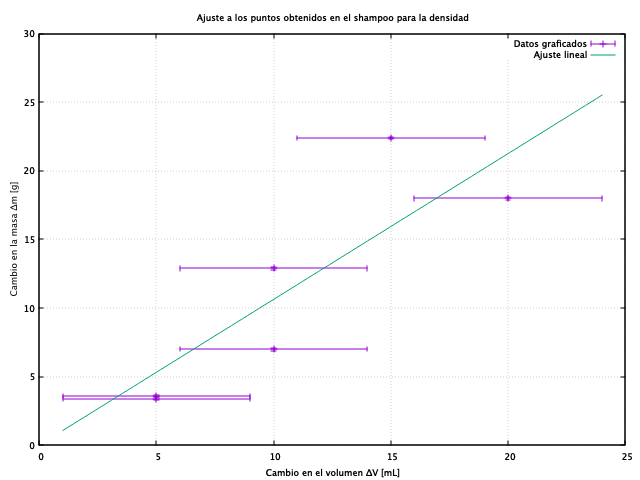
\includegraphics[width=12cm]{Shampooden.png}
    \caption{Ajuste de una linea recta para obtener la razón $\Delta m / \Delta V$ en el shampoo.}
\end{figure}

Entonces $\frac{\Delta m}{\Delta V} = 1.06 \pm 0.13$ que resulta un valor aproximado a la densidad.


\subsubsection*{Glicerina.}% Table generated by Excel2LaTeX from sheet 'Sheet1'
\begin{table}[H]
  \centering
    \begin{tabular}{|c|c|c|c|c|c|c|} \hline
     & $V_i$ [mL] & $m_i$ [g] & $V_f$ [mL] & $m_f$ [g] & $\Delta V$ [mL] & $\Delta m$ [g] \\ \hline
    1     & $445\pm2$ & $710.00\pm0.05$ & $450.\pm2$ & $714.50\pm0.05$ & $5\pm4$ & $4.5\pm0.1$ \\ \hline
    2     & $445\pm2$ & $709.60\pm0.05$ & $450.\pm2$ & $713.20\pm0.05$ & $15\pm4$ & $3.6\pm0.1$ \\ \hline
    3     & $445\pm2$ & $708.60\pm0.05$ & $450.\pm2$ & $715.80\pm0.05$ & $20\pm4$ & $7.2\pm0.1$ \\ \hline
    4     & $445\pm2$ & $706.00\pm0.05$ & $450.\pm2$ & $717.30\pm0.05$ & $10\pm4$ & $11.3\pm0.1$ \\ \hline
    5     & $440.\pm2$ & $705.50\pm0.05$ & $455\pm2$ & $721.30\pm0.05$ & $5\pm4$ & $15.8\pm0.1$ \\ \hline
    6     & $440.\pm2$ & $703.50\pm0.05$ & $460.\pm2$ & $730.00\pm0.05$ & $10\pm4$ & $26.5\pm0.1$ \\ \hline
    \end{tabular}%
  \caption{Mediciones realizadas para la glicerina, se incluyen los datos iniciales, finales y una vez operados.}
\end{table}%

\begin{table}[H]
  \centering
    \begin{tabular}{|c|c|c|c|} \hline
          & $F_E$ [N] & $\Delta W$ & $| F_E - \Delta W |$ \\ \hline
    1     & $0.04\pm0.04$ & $0.044\pm0.001$ & 0.0009 \\ \hline
    2     & $0.04\pm0.04$ & $0.035\pm0.001$ & 0.0007 \\ \hline
    3     & $0.07\pm0.04$ & $0.070\pm0.001$ & 0.0014 \\ \hline
    4     & $0.11\pm0.04$ & $0.110\pm0.001$ & 0.0022 \\ \hline
    5     & $0.16\pm0.04$ & $0.154\pm0.001$ & 0.0031 \\ \hline
    6     & $0.26\pm0.04$ & $0.259\pm0.001$ & 0.0052 \\ \hline
    \end{tabular}%
  \caption{Cambio en el peso y fuerza de empuje para la glicerina y su comparación.}
\end{table}%


\begin{table}[H]
  \centering
    \begin{tabular}{|c|c|c|} \hline
          & $\Delta W$ [N] & $\rho_{gli}$ [g/mL]  \\ \hline
    1     & $0.044\pm0.001$ & $0.9\pm0.1$  \\ \hline
    2     & $0.035\pm0.001$ & $0.24\pm0.09$  \\ \hline
    3     & $0.070\pm0.001$ & $0.4\pm0.2$  \\ \hline
    4     & $0.110\pm0.001$ & $1.2\pm0.3$  \\ \hline
    5     & $0.154\pm0.001$ & $3.1\pm0.4$  \\ \hline
    6     & $0.259\pm0.001$ & $2.6\pm0.6$  \\ \hline
    \end{tabular}%
  \caption{Densidad de la glicerina a partir del cambio de peso.}
\end{table}%

Al ajustarle una recta $y = a*x$. Obtenemos que la pendiente es: $a = 1.0 \pm 0.4$.
\begin{figure}[H]
    \centering
    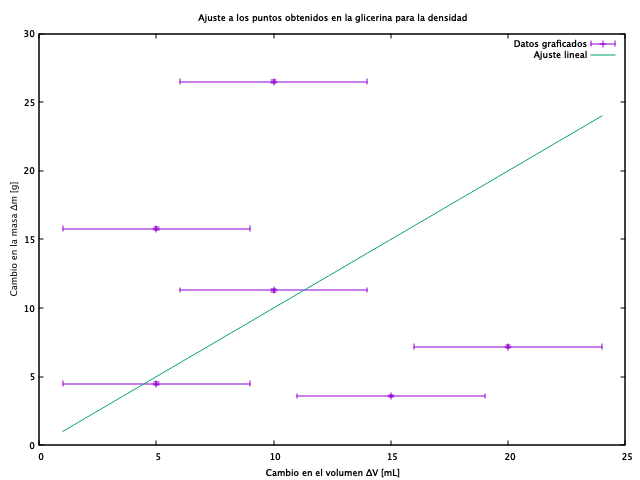
\includegraphics[width=12cm]{Glicerinaden.png}
    \caption{Ajuste de una linea recta para obtener la razón $\Delta m / \Delta V$ en la glicerina.}
\end{figure}

Entonces $\frac{\Delta m}{\Delta V} = 1.0 \pm 0.4$.





\subsubsection*{Aceite de oliva.}
% Table generated by Excel2LaTeX from sheet 'Sheet1'
\begin{table}[H]
  \centering
    \begin{tabular}{|c|c|c|c|c|c|c|} \hline
     & $V_i$ [mL] & $m_i$ [g] & $V_f$ [mL] & $m_f$ [g] & $\Delta V$ [mL] & $\Delta m$ [g] \\ \hline
    1     & $460\pm2$ & $577.30\pm0.05$ & $480.\pm2$ & $590.90\pm0.05$ & $20\pm4$ & $13.6\pm0.1$ \\ \hline
    2     & $455\pm2$ & $576.10\pm0.05$ & $470.\pm2$ & $589.50\pm0.05$ & $15\pm4$ & $13.4\pm0.1$ \\ \hline
    3     & $455\pm2$ & $575.40\pm0.05$ & $460.\pm2$ & $578.20\pm0.05$ & $5\pm4$ & $2.8\pm0.1$ \\ \hline
    4     & $455\pm2$ & $575.10\pm0.05$ & $465\pm2$ & $581.50\pm0.05$ & $10\pm4$ & $6.4\pm0.1$ \\ \hline
    5     & $455\pm2$ & $573.00\pm0.05$ & $460.\pm2$ & $574.70\pm0.05$ & $5\pm4$ & $1.7\pm0.1$ \\ \hline
    6     & $455\pm2$ & $572.80\pm0.05$ & $475\pm2$ & $590.30\pm0.05$ & $20\pm4$ & $17.5\pm0.1$ \\ \hline
    \end{tabular}%
  \caption{Mediciones realizadas para el aceite de oliva, se incluyen los datos iniciales, finales y una vez operados.}
\end{table}%

Y aquí la comparativa entre la diferencia en peso con el empuje:
\begin{table}[H]
  \centering
    \begin{tabular}{|c|c|c|c|} \hline
          & $F_E$ [N] & $\Delta W$ & $| F_E - \Delta W |$ \\ \hline
    1     & $0.03\pm0.04$ & $0.033\pm0.001$ & 0.0007 \\ \hline
    2     & $0.22\pm0.04$ & $0.219\pm0.001$ & 0.0044 \\ \hline
    3     & $0.18\pm0.04$ & $0.176\pm0.001$ & 0.0035 \\ \hline
    4     & $0.13\pm0.04$ & $0.126\pm0.001$ & 0.0025 \\ \hline
    5     & $0.04\pm0.04$ & $0.035\pm0.001$ & 0.0007 \\ \hline
    6     & $0.07\pm0.04$ & $0.068\pm0.001$ & 0.0014 \\ \hline
    \end{tabular}%
  \caption{Cambio en el peso y fuerza de empuje para el aceite de oliva.}
\end{table}%



\begin{table}[H]
  \centering
    \begin{tabular}{|c|c|c|} \hline
          & $\Delta W$ [N] & $\rho_{Ac} [g/mL]$ \\ \hline
    1     & $0.033\pm0.001$ & $0.17\pm0.09$  \\ \hline
    2     & $0.219\pm0.001$ & $1.5\pm0.5$  \\ \hline
    3     & $0.176\pm0.001$ & $3.6\pm0.4$  \\ \hline
    4     & $0.126\pm0.001$ & $1.3\pm0.3$  \\ \hline
    5     & $0.035\pm0.001$ & $0.71\pm0.09$  \\ \hline
    6     & $0.068\pm0.001$ & $0.3\pm0.2$  \\ \hline
    \end{tabular}%
  \caption{Densidad del aceite de oliva en base a la diferencia de pesos}
\end{table}%

Al ajustarle una recta $y = a*x$. Obtenemos que $a = 1.06 \pm 0.13$.
\begin{figure}[H]
    \centering
    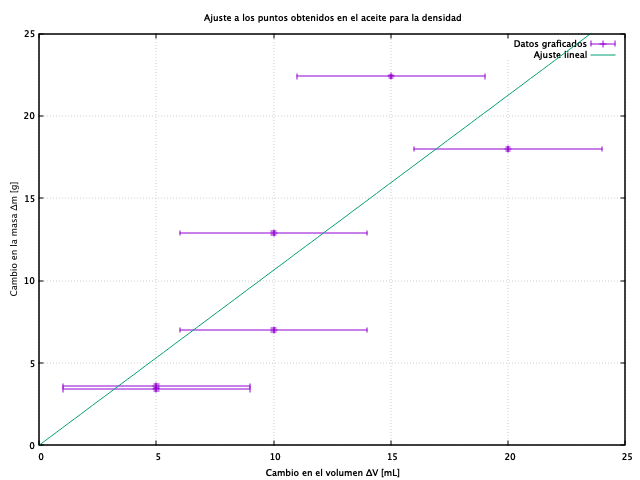
\includegraphics[width=12cm]{Aceiteden.png}
    \caption{Ajuste de una linea recta para obtener la razón $\Delta m / \Delta V$ en el aceite.}
\end{figure}

Entonces $\frac{\Delta m}{\Delta V} = 1.06 \pm 0.13$.

\section*{Conclusiones.}
\subsection*{Primer experimento.}
Los resultados muestran que, efectivamente, el cambio de peso del sistema se debe a un incremento en la fuerza de empuje. Esta fuerza de empuje incrementa al momento de permitir el flujo de aire de la botella al globo; el globo se infla, aumenta el volumen del sistema y la fuerza de empuje incrementa su magnitud, contrarrestando parcialmente los efectos de la gravedad y resultando en un ''cambio de masa'' medido en un instrumento que en realidad mide peso (La balanza).

Para obtener datos mas precisos sobre el volumen de aire contenido en el globo se propone tener una probeta con una graduación más fina, sin sacrificar la capacidad total de la misma. En este experimento no se considera como limitante la graduación de la probeta.

La segunda medición se salió de la separación normal, resultando en una diferencia de $1.2\pm0.2$ que creemos que, al igual que en la cuarta medida, todavía se estaba comprendiendo el sistema de medición;  conforme más medidas se realizaron, las incertidumbres de diferencia se fueron acercando a valores de 0.3 a 0.4 y con incertidumbre de 0.1 a 0.2. Esto refleja un mejor uso de los instrumentos, lo cual se traduce en una mejor precisión en las medidas obtenidas.

\subsection*{Segundo experimento.}
Debido a la resolución del instrumento de medición de volumen, los datos obtenidos para la densidad y sus incertidumbres terminan siendo intervalos muy grandes los cuales a pesar de siempre contener al valor teórico, no nos son útiles y hablan sobre un claro error en la elección de instrumentos a utilizar. Se podrían hacer varias mediciones más para observar si los valores tienden a un punto ya que se espera que este experimento sea reproducible; sin embargo, esto no ayudaría a reducir la incertidumbre asociada al cálculo. Es por ello que para hacer una mejor aproximación de la densidad del fluido en la probeta sería necesario hacer todas las mediciones  con una probeta de resolución una resolución mayor o aprovechar el aspecto de los cuerpos utilizados fueron sólidos con formas geométricas regulares de los cuales existen fórmulas para obtener dicho volumen.

En cuanto a resultados numéricos se obtiene que en general varían las fuerzas por centésimas de Newton si no consideramos la incertidumbre, el valor central que se espera es concordante con lo propuesto con Arquímedes, además de ello ya que son cercanos a lo que se propone, es posible obtener la relación $\rho = \frac{\Delta W}{Vg}$ y con ello valores para las densidades de los líquidos que se utilizaron: $\rho_{shampoo} = 1.06\pm0.13g/cm^3$ comparado con el medido con un densímetro de $\rho_{s} = 1.030\pm0.005 g/cm^3$, $\rho_{glicerina} = 1.0\pm0.4 g/cm^3$ comparado con el medido con un densímetro de $\rho_{g} = 1.260\pm0.005 g/cm^3$ y $\rho_{aceite} = 1.06\pm0.13 g/cm^3$ comparado con $\rho_{a} = 0.910 \pm 0.005 g/cm^3$. Pero esto sería abusar de la incertidumbre puesto que la despreciamos lo cual vuelve dudosos los resultados.

En general se presenta un gran problema en cualquier dato relacionado y/o obtenido a partir del volumen puesto que al haber restado dos cantidades podemos observar que en los volúmenes con valor de 5 mL esta forma de medición hacía que dicho valor contase con un 80\% de incertidumbre lo cual vuelve prácticamente inútil a la medida obtenida y en particular si observamos el caso de la relación obtenida entre el peso y volumen para obtener la densidad, esta incertidumbre asociada al volumen comprende un gran problema puesto que al propagarse amplia el rango.

De esta forma aunque resultan prometedores los datos obtenidos de este experimento, la elección incorrecta y mala planeación del diseño experimental llevaron a resultados que, inequívocamente, son perfectibles desde el punto de vista resolutivo, es decir mejorable en aspectos relacionados a la incertidumbre y que por medio de modificaciones simples permitan observar resultados fiables que verifiquen la relación entre diferencia de peso con la fuerza de empuje y poder obtener resultados secundarios como las densidades de un fluido.













\begin{thebibliography}{a}
\bibitem{pradery} \textsc{Resnick, R., Halliday, D., Krane, K.} (2001). \textit{Física Vol. 1}. ($4^a$ ed). México. GRUPO PATRIA CULTURAL,

\bibitem{pradery} \textsc{Bevington P., Robinson D.} (1969). \textit{Data Reduction and Error Analysis for the Physical Sciences
}. ($3^a$ ed). México. Mc Graw Hill.

\bibitem{pradery} \textsc{INN} (2011). \textit{CALCULO DE LA ACELERACIÓN LOCAL DE GRAVEDAD} [en linea]. Primera edición [ebook]. Santiago de Chile, Chile: Instituto Nacional de Normalización (Chile). Recuperado 3 de octubre de 2019 en \url{http://www.metrologia.cl/medios/noticias/GRAVEDAD_EN_CHILE.pdf}

\bibitem{pradery} \textsc{Zwiefelhofer D.} (2008).
\textit{19 N 99 W. findlatitudeandlongitude} [en linea]. Recuperado 3 de octubre de 2019 en \url{https://www.findlatitudeandlongitude.com/?loc=19+N+99+W&id=519829}

\bibitem{pradery} \textsc{s.a.} (2013).
\textit{Ciudad de México} [en linea]. Recuperado 3 de octubre de 2019 en \url{https://es-mx.topographic-map.com/maps/60mt/Ciudad-de-M\%C3\%A9xico/ }

\bibitem{pradery} \textsc{Moreno Corral, M. A..} (2013).
\textit{Primeras mediciones precisas de la gravedad hechas en México. Rev. mex. fís. E} [en linea].  2014, vol.60, n.1 [citado  2019-10-02], pp.24-30. Recuperado 3 de octubre de 2019 en \url{http://www.scielo.org.mx/scielo.php?script=sci_arttext&pid=S1870-35422014000100007&lng=es&nrm=iso}. ISSN 1870-3542.

\end{thebibliography}

\end{document}



